\begin{frame}
    \frametitle{\problemtitle}
    \begin{block}{Problem}
    	Given chains of various lengths, how many chain links do you need to open, interlock with other chain links and close again, to form a cyclic chain
    \end{block}
	\centering
	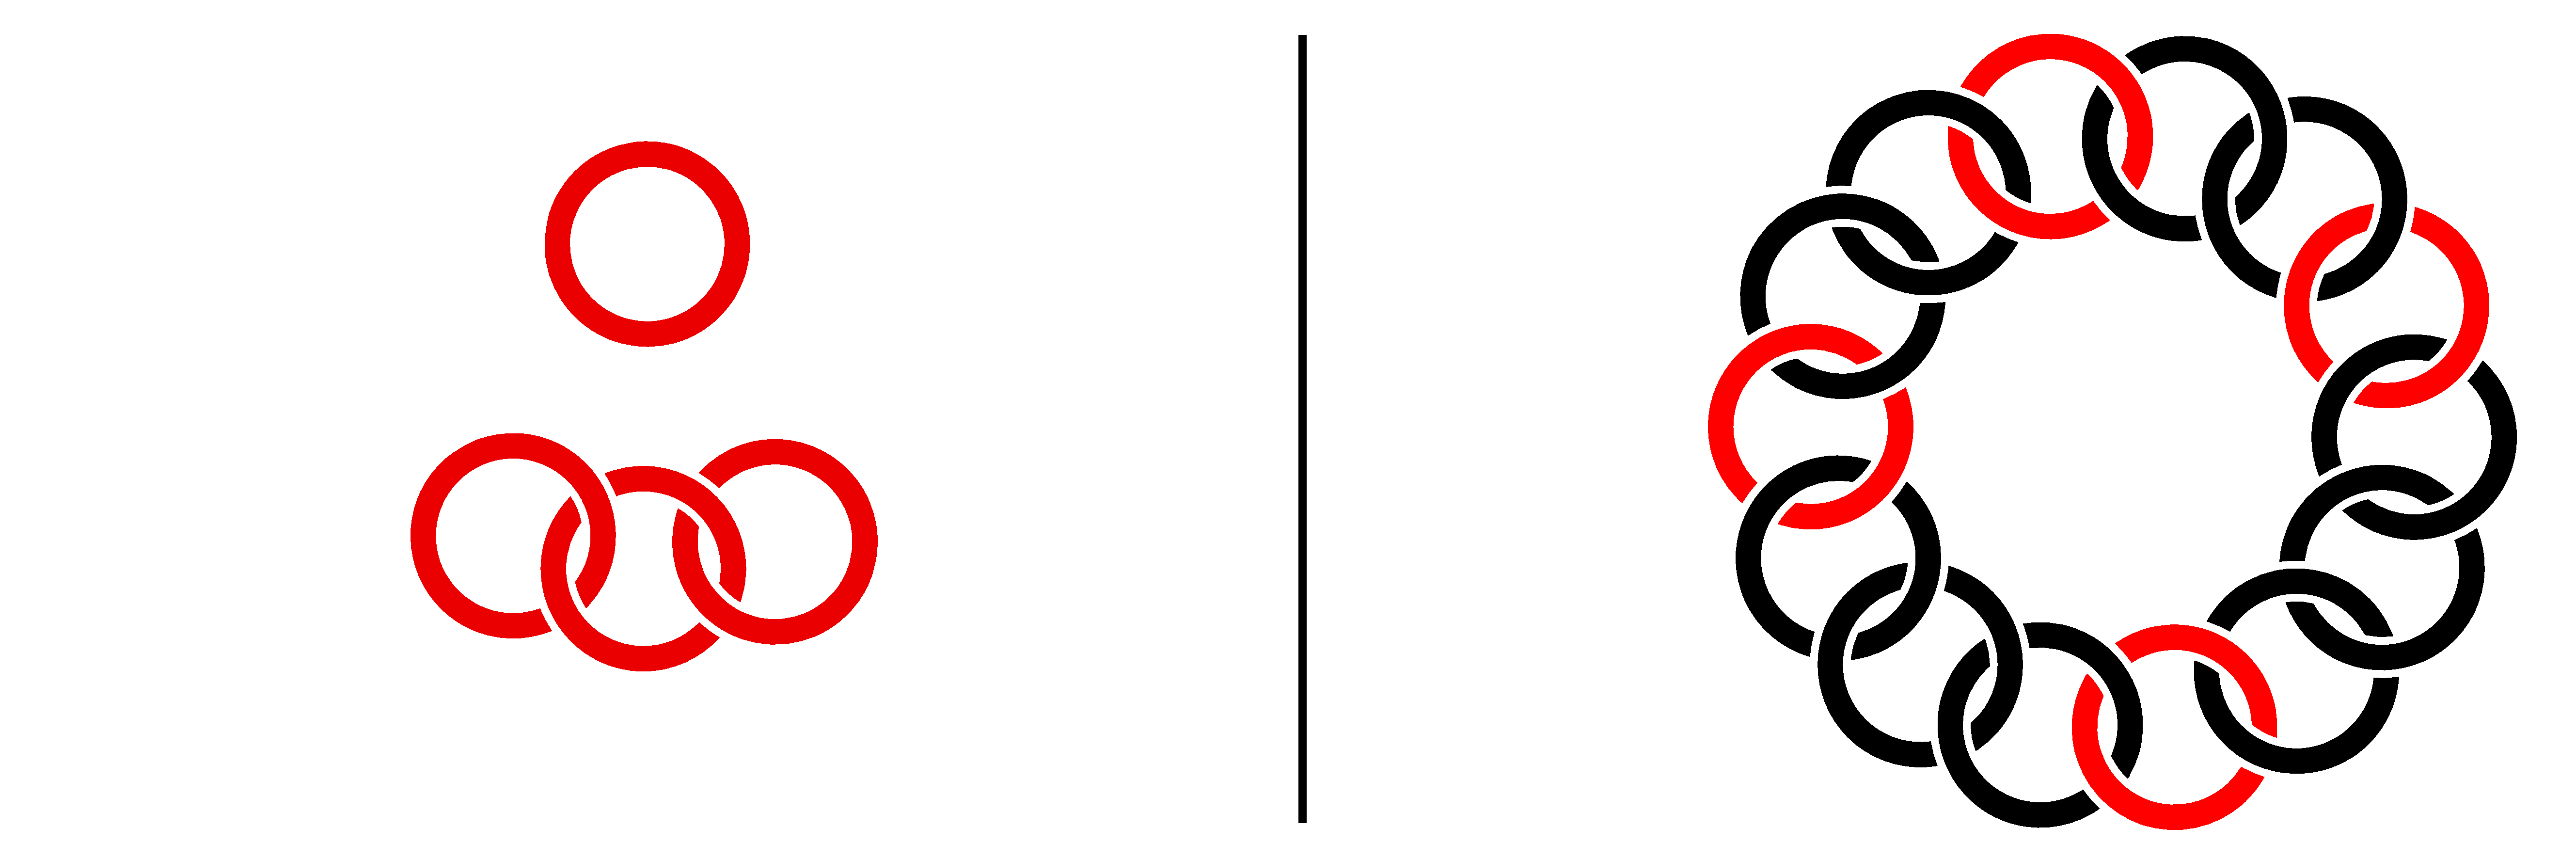
\includegraphics[width=0.5\textwidth]{example}
	\pause
    \begin{block}{Solution}
    	\begin{itemize}
    		\item You need to open $a$ chain links such that you end up with $b\leq a$ chains remaining
    		\pause
    		\item If $b>a$ You need to open more chain links
    		\pause
    		\item If you open chain links from the shortest chain you have the chance to completely use up a chain
    		\item This not only increases $a$ but also decreases $b$
    		\pause
    		\item[$\Rightarrow$] It is optimal to open chain links from the shortest chains first
    	\end{itemize}
    \end{block}
\end{frame}
